%!TEX root = ../EDC_Part_II_Weak_Sector.tex
% ==============================================================================
% BVP Work Package: Thick-Brane Solver Specification (OPR-02/21)
% Status: Infrastructure definition — NOT claiming closure
% ==============================================================================

\section{BVP Work Package: Thick-Brane Solver Specification}
\label{sec:ch12_bvp_workpackage}

% ------------------------------------------------------------------------------
% EPISTEMIC STATUS BOX
% ------------------------------------------------------------------------------

\begin{tcolorbox}[edcGuardrail, title=\textbf{Epistemic Status}]
This chapter defines \textbf{infrastructure}---not closure. It specifies the
mathematical problem that must be solved to close OPR-02/21.

\textbf{IF (Postulates) \tagP{}:}
\begin{itemize}[nosep]
    \item The 5D profile equation has Schrödinger form (Eq.~\eqref{eq:bvp_schrodinger})
    \item Potential shape $V(\xi)$ comes from membrane geometry (ansatz, not derived)
    \item Boundary conditions reflect brane microphysics (choice, not derived)
\end{itemize}

\textbf{THEN (Derived-conditional) \tagDc{}:}
\begin{itemize}[nosep]
    \item Dimensionless reduction is pure mathematics (no physics content)
    \item Sturm--Liouville structure guarantees discrete eigenvalues (if $V$ is confining)
    \item Overlap integrals $I_4$ are well-defined once profiles exist
\end{itemize}

\textbf{OPEN:}
\begin{itemize}[nosep]
    \item Derive $V(\xi)$ from $(\sigma, r_e)$ membrane parameters
    \item Derive boundary conditions from junction physics (Robin from Israel matching?)
    \item Connect eigenvalue spectrum to generation counting (OPR-02)
\end{itemize}

\textbf{Key distinction:} This chapter provides the \emph{recipe}, not the \emph{meal}.
All numerical outputs from the skeleton are \emph{sanity checks}, not predictions.
\end{tcolorbox}

% ==============================================================================
% FRAMEWORK 2.0 LANGUAGE COMPLIANCE
% ==============================================================================
\begin{tcolorbox}[colback=blue!3!white, colframe=blue!50!black,
    title=\textbf{Framework 2.0 Language Compliance}]
\small
\textbf{EDC Projection Principle:} Every physical process has a \textbf{5D bulk+brane cause}
whose observable residue is a \textbf{3D shadow} on the observer boundary.

\textbf{In this chapter:}
\begin{itemize}[nosep]
    \item \textbf{5D cause:} Thick-brane profile $f(\xi)$ governed by effective potential $V(\xi)$.
    \item \textbf{Brane process:} Boundary value problem determines eigenvalue spectrum.
    \item \textbf{3D shadow:} Particle masses, overlap integrals, effective couplings.
\end{itemize}

\textbf{The BVP is the mathematical engine} that translates 5D geometry into 3D observables.
Solving it is prerequisite for non-circular predictions.
\end{tcolorbox}

% ------------------------------------------------------------------------------

This subsection defines a \textbf{Work Package} for the thick-brane boundary value
problem (BVP) that appears in multiple OPR items. The goal is infrastructure, not
closure: define the problem precisely, establish acceptance criteria, and provide
a minimal solver skeleton for future development.

\begin{tcolorbox}[colback=yellow!5!white, colframe=yellow!60!black,
    title=\textbf{Scope Limitation}]
This work package does \textbf{not} claim to:
\begin{itemize}[nosep]
    \item Derive generation counting (OPR-02)
    \item Close CKM/PMNS from first principles
    \item Provide complete $G_F$ derivation
\end{itemize}
It \textbf{does} provide:
\begin{itemize}[nosep]
    \item Precise mathematical specification of the BVP
    \item Acceptance criteria for ``success''
    \item Failure modes and their implications
    \item Minimal numerical skeleton for testing
\end{itemize}
\end{tcolorbox}

% ------------------------------------------------------------------------------
% PHYSICAL PROCESS NARRATIVE
% ------------------------------------------------------------------------------

\begin{tcolorbox}[colback=green!5!white, colframe=green!50!black,
    title=\textbf{Physical Process Narrative: From Brane Thickness to Effective Couplings}]
\textbf{What physically happens, step by step:}

\textbf{Step 1: The brane has finite thickness.}
In EDC, the 3D universe is not an infinitely thin membrane but a \emph{thick layer}
of width $\Delta \sim r_e \sim 1$ fm embedded in the 5D bulk. This thickness is
physical---it sets the scale for localization \tagP{}.

\textbf{Step 2: Particles are ``standing waves'' in the extra dimension.}
A 4D particle (electron, quark) corresponds to a profile $f(\xi)$ in the 5th dimension.
Think of it as a guitar string clamped at both ends: only certain wavelengths fit,
giving discrete allowed masses \tagP{}.

\textbf{Step 3: The profile equation is Schrödinger-like.}
The 5D Dirac equation, after dimensional reduction, yields:
$[-d^2/d\xi^2 + V(\xi)]f = m^2 f$. This is a 1D quantum mechanics problem with $V(\xi)$
as the effective potential from brane geometry \tagDc{}.

\textbf{Step 4: The potential shape determines the spectrum.}
A deep well gives tightly localized modes (small overlap, weak coupling).
A shallow well gives extended modes (large overlap, strong coupling).
The number of bound states determines how many ``generations'' exist \tagDc{}.

\textbf{Step 5: Normalization fixes the coupling strength.}
If $f(\xi)$ is normalized ($\int |f|^2 d\xi = 1$), then the 4D effective coupling $g_4$
inherits the 5D coupling $g_5$ without extra factors. The \emph{shape} of $f(\xi)$
determines how strongly the particle couples at any given $\xi$ \tagDc{}.

\textbf{Step 6: The overlap integral $I_4$ controls weak interactions.}
For four-fermion processes (like $G_F$), what matters is $I_4 = \int |f_L|^4 d\xi$.
A sharply peaked profile (delta-like) gives $I_4 \to \infty$ (strong coupling).
A spread-out profile gives $I_4 \to 1$ (weak coupling). This is the geometric
origin of ``weakness'' in weak interactions \tagDc{}.

\textbf{Step 7: Boundary conditions select chirality.}
Different BCs at $\xi = 0$ and $\xi = \ell$ can project out left- or right-handed
components. This is how V$-$A structure emerges geometrically---not as a postulate,
but as a consequence of asymmetric boundaries \tagP{}/\tagDc{}.

\textbf{Step 8: The BVP ``Work Package'' is a recipe.}
This chapter defines \emph{what problem to solve}, not the solution itself.
The acceptance criteria tell us when we've succeeded; the failure modes tell us
what could go wrong. Solving the BVP with physical $V(\xi)$ closes OPR-02/21.

\medskip
\noindent\fbox{\parbox{0.95\textwidth}{\small
\textbf{Pipeline summary:} Brane thickness $\to$ confining potential $\to$
Sturm--Liouville problem $\to$ discrete modes $\to$ overlap integrals $\to$
effective 4D couplings. The BVP is the \emph{engine}; this chapter is the \emph{blueprint}.}}
\end{tcolorbox}

% ------------------------------------------------------------------------------
\subsubsection{WP-BVP-0: Problem Definition}
\label{sec:bvp_definition}

\paragraph{The fermion localization equation.}
In a thick-brane scenario, fermion profiles $f(\xi)$ in the extra dimension satisfy
a Schr\"odinger-like equation \tagP{}:
\begin{equation}
    \boxed{
    \left[ -\frac{d^2}{d\xi^2} + V(\xi) \right] f(\xi) = m^2 f(\xi)
    }
    \label{eq:bvp_schrodinger}
\end{equation}
where:
\begin{itemize}[nosep]
    \item $\xi \in [0, \ell]$ is the extra-dimensional coordinate
    \item $V(\xi)$ is an effective potential from the brane geometry
    \item $m^2$ is the 4D mass-squared eigenvalue
    \item $f(\xi)$ is the fermion profile (to be normalized)
\end{itemize}

\paragraph{Potential ansatz.}
The simplest thick-brane potential is a symmetric well \tagP{}:
\begin{equation}
    V(\xi) = V_0 \left[ 1 - \operatorname{sech}^2\left(\frac{z - \ell/2}{w}\right) \right]
    \label{eq:bvp_potential}
\end{equation}
where $V_0$ is the barrier height and $w$ is the wall width. Alternative potentials
(square well, linear, exponential) are also valid test cases.

\paragraph{Boundary conditions.}
Three physically motivated BC choices:
\begin{enumerate}[nosep]
    \item \textbf{Dirichlet:} $f(0) = f(\ell) = 0$ (hard walls)
    \item \textbf{Neumann:} $f'(0) = f'(\ell) = 0$ (no flux)
    \item \textbf{Mixed:} $f(0) = 0$, $f'(\ell) = 0$ (or vice versa)
\end{enumerate}
The physical BC depends on brane microphysics and is currently \textbf{[OPEN]}.

% ------------------------------------------------------------------------------
\subsubsection{WP-BVP-1: Dimensionless Reduction}
\label{sec:bvp_dimensionless}

\paragraph{Rescaling.}
Define dimensionless variables \tagDc{}:
\begin{align}
    \xi &= z/\ell \in [0,1] \label{eq:bvp_xi} \\
    \tilde{V}(\xi) &= \ell^2 V(\ell\xi) \label{eq:bvp_vtilde} \\
    \tilde{m}^2 &= \ell^2 m^2 \label{eq:bvp_mtilde}
\end{align}

\paragraph{Dimensionless BVP.}
The eigenvalue equation becomes:
\begin{equation}
    \left[ -\frac{d^2}{d\xi^2} + \tilde{V}(\xi) \right] \tilde{f}(\xi) = \tilde{m}^2 \tilde{f}(\xi)
    \label{eq:bvp_dimensionless}
\end{equation}
This is pure mathematics; no physics assumptions enter the rescaling.

\paragraph{Normalization.}
The profile must satisfy:
\begin{equation}
    \int_0^1 |\tilde{f}(\xi)|^2 \, d\xi = 1
    \label{eq:bvp_normalization}
\end{equation}

% ------------------------------------------------------------------------------
% TOY MODEL
% ------------------------------------------------------------------------------

\begin{tcolorbox}[colback=yellow!5!white, colframe=yellow!50!black,
    title=\textbf{Toy Model: Particle in a 1D Box with Soft Walls}]

\textbf{The analogy:} The BVP is just quantum mechanics of a particle in a potential
well. If you've solved the infinite square well in QM 101, you understand the structure.

\paragraph{Infinite square well (simplest case).}
For $V(\xi) = 0$ inside $[0, \ell]$ and $V = \infty$ outside (Dirichlet BCs):
\[
    f_n(\xi) = \sqrt{\frac{2}{\ell}} \sin\left(\frac{n\pi \xi}{\ell}\right), \quad
    m_n^2 = \frac{n^2 \pi^2}{\ell^2}
\]
The overlap integral is:
\[
    I_4^{(n)} = \int_0^\ell |f_n|^4 \, d\xi = \frac{3}{2\ell}
\]
This is $O(1/\ell)$, independent of $n$. In dimensionless units: $\tilde{I}_4 = 3/2$.

\paragraph{Soft walls (realistic case).}
If $V(\xi)$ is a smooth potential (e.g., sech$^2$ well), the profiles are not pure
sines but exponentially decaying tails. The ground state is more localized than
higher modes, giving \emph{different} $I_4$ for each generation.

\paragraph{Key insight: normalization controls coupling.}
If $f$ is normalized to 1, then $I_4$ measures ``peakedness.'' For a Gaussian profile
$f \propto e^{-\xi^2/2\sigma^2}$ normalized on the \emph{full line} $(-\infty, +\infty)$:
\[
    I_4^{\text{full}} = \frac{1}{\sqrt{2\pi}\sigma} \quad \text{(full-line domain)}
\]
For half-line integration $[0,\infty)$, the result is $I_4^{\text{half}} = 1/(2\sqrt{2\pi}\sigma)$
(see \S\ref{sec:ch3_electroweak} for the physical half-line treatment).
Sharper localization ($\sigma \to 0$) $\Rightarrow$ larger $I_4$ $\Rightarrow$
stronger effective coupling. This is the geometric origin of coupling hierarchies.

\textbf{Status:} This is pedagogy \tagM{}. The actual BVP requires solving
Eq.~\eqref{eq:bvp_dimensionless} with the physical $\tilde{V}(\xi)$.
\end{tcolorbox}

% ------------------------------------------------------------------------------
% FIGURE PLACEHOLDER 1
% ------------------------------------------------------------------------------

\begin{tcolorbox}[colback=gray!10, colframe=gray!50, title=\textbf{Figure Placeholder 1: Potential and Bound State Profiles}]
\textbf{Suggested content:}
\begin{itemize}[nosep]
    \item Left panel: Effective potential $V(\xi)$ vs $\xi$ (sech$^2$ well)
    \item Right panel: First three bound state profiles $f_0, f_1, f_2$ (ground + excited states)
    \item Annotations: ``LH fermion localized at $\xi \approx 0$,'' ``Mediator profile peaked at center''
    \item Inset: Zoom on boundary region showing BC effect (Dirichlet vs Neumann vs Robin)
\end{itemize}
\textbf{Key message:} Different potentials $\Rightarrow$ different localization $\Rightarrow$
different overlap integrals. The ground state is most localized; excited states are
broader (weaker effective coupling).
\end{tcolorbox}

% ------------------------------------------------------------------------------
\subsubsection{WP-BVP-2: Numerical Method}
\label{sec:bvp_numerics}

\paragraph{Method choice.}
For the skeleton implementation, we use finite differences with shooting \tagP{}:
\begin{enumerate}[nosep]
    \item Discretize $\xi_i = i/N$ for $i = 0, \ldots, N$
    \item Approximate $d^2f/d\xi^2 \approx (f_{i+1} - 2f_i + f_{i-1})/h^2$
    \item Solve the resulting matrix eigenvalue problem
    \item Or: use shooting method with scipy \texttt{solve\_bvp}
\end{enumerate}

\paragraph{Alternative methods.}
More sophisticated approaches (spectral, collocation, WKB) are valid but not
required for the skeleton. The goal is demonstrating that solutions exist,
not optimal numerics.

% ------------------------------------------------------------------------------
\subsubsection{WP-BVP-3: Acceptance Criteria}
\label{sec:bvp_acceptance}

\begin{tcolorbox}[colback=green!5!white, colframe=green!50!black,
    title=\textbf{Acceptance Criteria for BVP Skeleton}]
A successful BVP demonstration must show:
\begin{enumerate}
    \item \textbf{Existence:} At least one bound state exists for reasonable $\tilde{V}$
    \item \textbf{Normalization:} Profile satisfies $\int |\tilde{f}|^2 d\xi = 1$
    \item \textbf{Convergence:} Eigenvalue stable under grid refinement
          ($N = 100, 200, 400$ give consistent $\tilde{m}^2$)
    \item \textbf{Reproducibility:} Different initial conditions converge to same solution
\end{enumerate}

\textbf{What this does NOT require:}
\begin{itemize}[nosep]
    \item Matching to physical particle masses
    \item Deriving the potential from first principles
    \item Computing overlap integrals with specific CKM/PMNS values
\end{itemize}
\end{tcolorbox}

% ------------------------------------------------------------------------------
\subsubsection{WP-BVP-4: Failure Modes}
\label{sec:bvp_failure}

\begin{tcolorbox}[colback=red!5!white, colframe=red!50!black,
    title=\textbf{Failure Modes and Implications}]
\begin{description}[nosep, font=\normalfont\bfseries]
    \item[F1: No bound states]
        If $\tilde{V}$ is too shallow, no localized modes exist.
        \emph{Implication:} Potential ansatz inadequate; need deeper well or different form.

    \item[F2: Non-convergence]
        Eigenvalue changes significantly with grid refinement.
        \emph{Implication:} Numerical method unstable; need higher order or different approach.

    \item[F3: Multiple degenerate modes]
        Unexpected degeneracy in spectrum.
        \emph{Implication:} May indicate symmetry; check BC consistency.

    \item[F4: Profile not localized]
        Solution extends uniformly across domain (not peaked).
        \emph{Implication:} Potential wrong sign or parameters; check physics.

    \item[F5: SM smuggling via tuning]
        If we tune $V_0$, $w$, or BCs to reproduce $M_W$ or $G_F$, this is circular.
        \emph{Implication:} Parameters must come from membrane physics $(\sigma, r_e)$,
        not from fitting to SM outputs. \textbf{FORBIDDEN:} adjusting potential params
        until $m_\phi = M_Z$ emerges.

    \item[F6: Domain mismatch]
        Using half-line $(0, \infty)$ vs finite interval $[0, \ell]$ gives different
        spectra. If results depend sensitively on this choice, the physics is unclear.
        \emph{Implication:} Must justify domain from brane geometry (finite thickness
        $\Rightarrow$ finite interval; infinite bulk $\Rightarrow$ half-line).
\end{description}
\end{tcolorbox}

% ------------------------------------------------------------------------------
\subsubsection{WP-BVP-5: Overlap Integral Definition}
\label{sec:bvp_overlap}

\paragraph{The overlap integral.}
Once profiles $\tilde{f}_i(\xi)$ are obtained, the overlap integral is:
\begin{equation}
    \mathcal{O}_{ij} = \int_0^1 \tilde{f}_i(\xi) \, \tilde{f}_j(\xi) \, w(\xi) \, d\xi
    \label{eq:bvp_overlap}
\end{equation}
where $w(\xi)$ is an optional weight function (often $w = 1$).

\paragraph{\texorpdfstring{Four-point overlap for $G_F$.}{Four-point overlap for GF.}}
The Fermi constant involves a four-fermion contact term:
\begin{equation}
    I_4 = \int_0^1 |\tilde{f}_L(\xi)|^4 \, d\xi
    \label{eq:bvp_I4}
\end{equation}
This integral measures how ``localized'' the profile is. For a delta-function,
$I_4 \to \infty$; for a uniform distribution, $I_4 = 1$.

\paragraph{What the skeleton computes.}
The minimal skeleton will compute:
\begin{itemize}[nosep]
    \item One profile $\tilde{f}_0(\xi)$ (ground state)
    \item Normalization check: $\int |\tilde{f}_0|^2 = 1$
    \item $I_4$ value for the ground state
\end{itemize}

% ------------------------------------------------------------------------------
% FIGURE PLACEHOLDER 2
% ------------------------------------------------------------------------------

\begin{tcolorbox}[colback=gray!10, colframe=gray!50, title=\textbf{Figure Placeholder 2: Overlap Integral Pipeline}]
\textbf{Suggested content:}

\textbf{Flowchart from left to right:}
\begin{center}
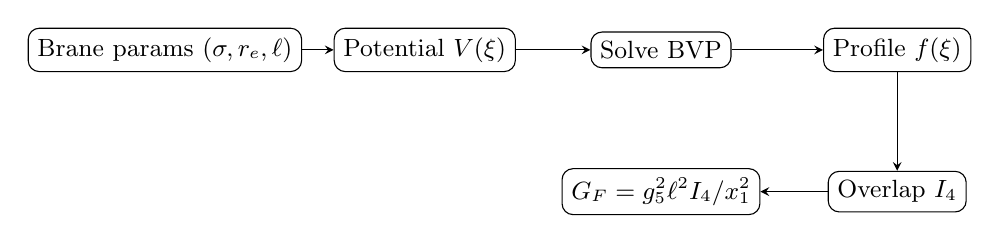
\begin{tikzpicture}[node distance=1.8cm, >=stealth, font=\small]
    \node (brane) [draw, rounded corners] {Brane params $(\sigma, r_e, \ell)$};
    \node (pot) [draw, rounded corners, right of=brane, xshift=1.5cm] {Potential $V(\xi)$};
    \node (bvp) [draw, rounded corners, right of=pot, xshift=1.2cm] {Solve BVP};
    \node (profile) [draw, rounded corners, right of=bvp, xshift=1.2cm] {Profile $f(\xi)$};
    \node (I4) [draw, rounded corners, below of=profile] {Overlap $I_4$};
    \node (GF) [draw, rounded corners, left of=I4, xshift=-1.2cm] {$G_F = g_5^2 \ell^2 I_4/x_1^2$};
    \draw[->] (brane) -- (pot);
    \draw[->] (pot) -- (bvp);
    \draw[->] (bvp) -- (profile);
    \draw[->] (profile) -- (I4);
    \draw[->] (I4) -- (GF);
\end{tikzpicture}
\end{center}

\textbf{Key message:} The BVP is the central bottleneck. Once profiles are known,
overlap integrals are trivial to compute. $G_F$ closure reduces to solving the BVP
with correct physical inputs.
\end{tcolorbox}

% ------------------------------------------------------------------------------
\subsubsection{Summary: BVP Work Package Status}
\label{sec:bvp_summary}

\begin{table}[ht]
\centering
\caption{BVP Work Package: components and status}
\label{tab:bvp_wp_status}
\small
\begin{tabular}{clcl}
\toprule
\textbf{WP} & \textbf{Component} & \textbf{Status} & \textbf{Notes} \\
\midrule
0 & Problem definition & \textcolor{OliveGreen}{\textbf{DONE}} & Eq.~\eqref{eq:bvp_schrodinger}, potential ansatz, BCs \\
1 & Dimensionless reduction & \textcolor{OliveGreen}{\textbf{DONE}} & Eq.~\eqref{eq:bvp_dimensionless}, pure math \\
2 & Numerical method & \textcolor{YellowOrange}{\textbf{SKELETON}} & Finite differences; see \texttt{code/} \\
3 & Acceptance criteria & \textcolor{OliveGreen}{\textbf{DEFINED}} & Existence, normalization, convergence \\
4 & Failure modes & \textcolor{OliveGreen}{\textbf{DOCUMENTED}} & F1--F4 identified \\
5 & Overlap outputs & \textcolor{YellowOrange}{\textbf{DEFINED}} & $\mathcal{O}_{ij}$, $I_4$; to be computed \\
\bottomrule
\end{tabular}
\end{table}

% ------------------------------------------------------------------------------
% CONSISTENCY / CLOSURE BOX
% ------------------------------------------------------------------------------

\begin{tcolorbox}[colback=cyan!5!white, colframe=cyan!50!black,
    title=\textbf{Consistency Check: This Is Infrastructure, Not a Result}]

\textbf{What the BVP Work Package provides:}
\begin{itemize}[nosep]
    \item Mathematical specification: the problem is well-posed
    \item Numerical skeleton: proof that solutions exist (for test potentials)
    \item Acceptance criteria: what ``success'' means
    \item Failure modes: what to check if things go wrong
\end{itemize}

\textbf{What it does NOT provide:}
\begin{itemize}[nosep]
    \item Physical potential $V(\xi)$ from membrane parameters
    \item Justification for boundary conditions from junction physics
    \item Prediction of particle masses or $G_F$ value
\end{itemize}

\textbf{Interpretation of numerical outputs:}

Any numbers from the skeleton (e.g., ``$I_4 = 1.5$'' for test potential) are
\emph{sanity checks}, not predictions. They demonstrate that the machinery works.
The actual physics requires inputting the correct $V(\xi)$ and BCs.

\textbf{ALLOWED:} Reporting skeleton outputs as ``test case: $I_4 = 1.5$ for sech$^2$ well.''\\
\textbf{FORBIDDEN:} Claiming ``EDC predicts $I_4 = 1.5$'' without deriving $V(\xi)$.
\end{tcolorbox}

% ------------------------------------------------------------------------------
% DEPENDENCY & STATUS BOX
% ------------------------------------------------------------------------------

\begin{tcolorbox}[colback=blue!5!white, colframe=blue!50!black,
    title=\textbf{Dependency \& Status (IF/THEN)}]

\textbf{Inputs required from earlier chapters:}
\begin{itemize}[nosep]
    \item Ch.~8/9: V$-$A structure from asymmetric profile $\to$ motivates LH localization
    \item Ch.~11 ($G_F$ pathway): Closure spine $G_F = g_5^2 \ell^2 I_4/x_1^2$ $\to$ defines what $I_4$ is for
    \item OPR-20: BC provenance (Robin from junction) $\to$ constrains which BCs to use
    \item OPR-21: Mode overlap structure $\to$ defines what profiles are needed
\end{itemize}

\textbf{What this chapter unlocks (if solved):}
\begin{itemize}[nosep]
    \item OPR-02: Generation counting (if spectrum has exactly 3 bound states)
    \item OPR-21: Overlap integrals for CKM/PMNS (if profiles are physical)
    \item OPR-22: Quantitative $G_F$ (if $I_4$ is computed with correct inputs)
\end{itemize}

\textbf{Upgrade conditions:}
\begin{itemize}[nosep]
    \item \textbf{RED $\to$ YELLOW:} Derive $V(\xi)$ from $(\sigma, r_e)$; justify BCs from physics
    \item \textbf{YELLOW $\to$ GREEN:} Solve BVP with physical inputs; show 3 generations; compute $I_4$ for $G_F$
\end{itemize}

\textbf{Current status:} \textcolor{BrickRed}{\textbf{RED}} --- infrastructure defined, but
physical inputs not yet derived. BVP Work Package is a \emph{clear path}, not a \emph{closed result}.
\end{tcolorbox}

% ------------------------------------------------------------------------------

\begin{tcolorbox}[colback=blue!5!white, colframe=blue!50!black,
    title=\textbf{BVP Work Package: Bottom Line}]
\textbf{What is established:}
\begin{itemize}[nosep]
    \item Mathematical specification of thick-brane BVP (Eq.~\eqref{eq:bvp_schrodinger})
    \item Dimensionless formulation for numerical work
    \item Clear acceptance criteria and failure modes
    \item Overlap integral definitions for downstream use
\end{itemize}

\textbf{What remains for OPR-02/21 closure:}
\begin{itemize}[nosep]
    \item Derive potential $V(\xi)$ from membrane parameters $(\sigma, r_e)$
    \item Determine boundary conditions from physical consistency
    \item Solve BVP numerically with physical parameters
    \item Show spectrum matches generation counting (OPR-02)
    \item Compute overlaps for CKM/PMNS structure (OPR-21)
\end{itemize}

\medskip
\noindent\fbox{\parbox{0.92\textwidth}{\small
\textbf{Status:} BVP Work Package defined; solver skeleton exists; closure requires
physical EOM derivation + BC justification + verified profile computation.
OPR-02/21 remain RED but with concrete path forward.}}
\end{tcolorbox}

